% STATUS: ACTIVE -- 2026-10-25 (user; renamed from 1025_wall_angle_estimator.tex): unified derivation of the wall-angle estimator in the measurement coordinate.
%   Sections 1-6: wall and motion gain matrix, process, process outputs, angle of a gain matrix, computed angle (six elements of A-hat,
%   angle theta(A-hat) after the update), estimated angle (10-25 option B: a_par, a_perp, slopes, theta as estimates; the six elements a-bar_m
%   compared with those of V(theta-hat) Lambda-hat V'(theta-hat); no angle measurement). Each form: true state, H, feedback, estimator,
%   dynamics of estimation errors (F_e, Q), angle. Section 7: fixed-point results (figures/fig_1025_fixed_{15,5}um.png from test_script/scratch/plot_1025_fixed.m, doc_mode = true, um_sel = [15 5]).
%   Section 8: angle error of the computed angle (element quality figures/fig_1025_a_quality.png from plot_1025_a_quality_doc.m, shown seeds =
%   the 3 with the smallest error, user 10-25, disclosed in the gray line; first-order sensitivity; figures/fig_1025_angle_err.png from
%   test_script/scratch/plot_1025_angle_err_doc.m).
%   Section 9: angle error of the estimated angle (figures/fig_1025_est_slow.png from test_script/scratch/plot_1025_est_slow_doc.m). H and the G_a relation of Section 6
%   checked by finite differences (10-25). The old Section 6 (theta_m from a-bar_m on top of six free elements) was redundant (memory
%   project_angle_state_redundant_2026-10-25) and is removed.
%   Rules: notation of memory project_notation_unified_2026-10-25 (fonts per TIE 2025: scalars italic; vectors / matrices bold upright
%   incl. Greek; lambda_c, delta, epsilon upright; hat = estimate and replaces the bar; subscript m = measured, keeps the bar);
%   presentation of memory feedback_angle_doc_presentation_2026-10-25 (derivation order, equations only with one gray line per block,
%   definitions as gray lines where first used, no numeric examples, no appendix, no abbreviations such as h, v, x[k]).
%   Supersedes as the main document: 1023_estimator_3d_xyz.tex, 1024_estimator_xyz_aprime.tex (kept until this one is complete).
%   Block diagram: figures/fig_1025_block.pdf (source figures/fig_1025_block.tex = test_results/figs_unused/blockdiag/block_two_forms.tex).
% Compile: xelatex 1025_computed_estimated_angle.tex (from reference/eq17_analysis/derivation/).
\documentclass[11pt,a4paper]{ctexart}
\usepackage[fleqn]{amsmath}
\usepackage{amssymb,bm,upgreek,graphicx}
\setlength{\mathindent}{0pt}
\usepackage{geometry}
\geometry{margin=1.8cm}
\setlength{\parindent}{0pt}
\setlength{\parskip}{0.2em}
\AtBeginDocument{\setlength{\abovedisplayskip}{4pt}\setlength{\belowdisplayskip}{4pt}}
\usepackage{xcolor}
\graphicspath{{figures/}}
\newcommand{\setline}[1]{\par\medskip\noindent{\small\textcolor[gray]{0.35}{#1}}}
\newcommand{\hd}[1]{\par\bigskip\noindent\underline{\textbf{#1}}}
% fonts: upright Greek scalars, bold upright vectors / matrices
\newcommand{\lc}{\lambda_c}
\newcommand{\dl}{\delta}
\newcommand{\bth}{\bm{\uptheta}}
\newcommand{\bep}{\bm{\upvarepsilon}_p}
\newcommand{\Lb}{\bar{\bm{\Lambda}}}
\newcommand{\Sn}{\bm{\Sigma}_n}
\newcommand{\Ab}{\bar{\mathbf A}}
\newcommand{\Ah}{\hat{\mathbf A}}
\newcommand{\Am}{\bar{\mathbf A}_m}
\newcommand{\av}{\bar{\mathbf a}}
\newcommand{\ah}{\hat{\mathbf a}}
\newcommand{\am}{\bar{\mathbf a}_m}
\newcommand{\dpb}{\dl\bar{\mathbf p}}
\newcommand{\dph}{\dl\hat{\mathbf p}}
\newcommand{\Fd}{\bar{\mathbf F}_{dp}}
\newcommand{\Mb}{\mathbf M}
\newcommand{\Mh}{\hat{\mathbf M}}
\newcommand{\I}{\mathbf I}
\newcommand{\V}{\mathbf V}
\newcommand{\Vh}{\hat{\mathbf V}}
\newcommand{\uu}{\mathbf u}
\newcommand{\vv}{\mathbf v}
\newcommand{\ww}{\mathbf w}
\newcommand{\wh}{\hat{\mathbf w}}
\newcommand{\apar}{\bar a_{\parallel}}
\newcommand{\aper}{\bar a_{\perp}}
\newcommand{\CK}{C_T\,\kappa_T}
\newcommand{\E}{\mathrm{E}}
\newcommand{\T}{T}
\newcommand{\GA}{\begin{bmatrix} F_x & 0 & 0 & F_y & F_z & 0 \\ 0 & F_y & 0 & F_x & 0 & F_z \\ 0 & 0 & F_z & 0 & F_x & F_y \end{bmatrix}}
\newcommand{\Jt}{\dfrac{\partial\bth}{\partial\av}\bigg|_{\Ah}}
\newcommand{\eyl}[1]{\big[\,\mathbf e_p^{\T}[k]\ \ \mathbf e_a^{\T}[k]#1\,\big]^{\T}}
\newcommand{\nv}{\big[\,\mathbf 0\ \ \mathbf 0\ \ -\bep^{\T}[k]\ \ \big(\hat{\mathbf a}'[k]\,\wh^{\T}[k]\,\bep[k]\big)^{\T}\ \ \mathbf 0\ \ \mathbf 0\,\big]^{\T}}
\newcommand{\Jw}{\dfrac{\partial\ww}{\partial\bth}\bigg|_{\hat\bth}}
\pagestyle{plain}

\begin{document}

\begin{center}\textbf{\large Computed angle and estimated angle of a tilted wall}\\[2pt]
\small 2026-10-25 \quad measurement coordinate $(x, y, z)$, local coordinate $(u, v, w)$\end{center}

\begin{center}
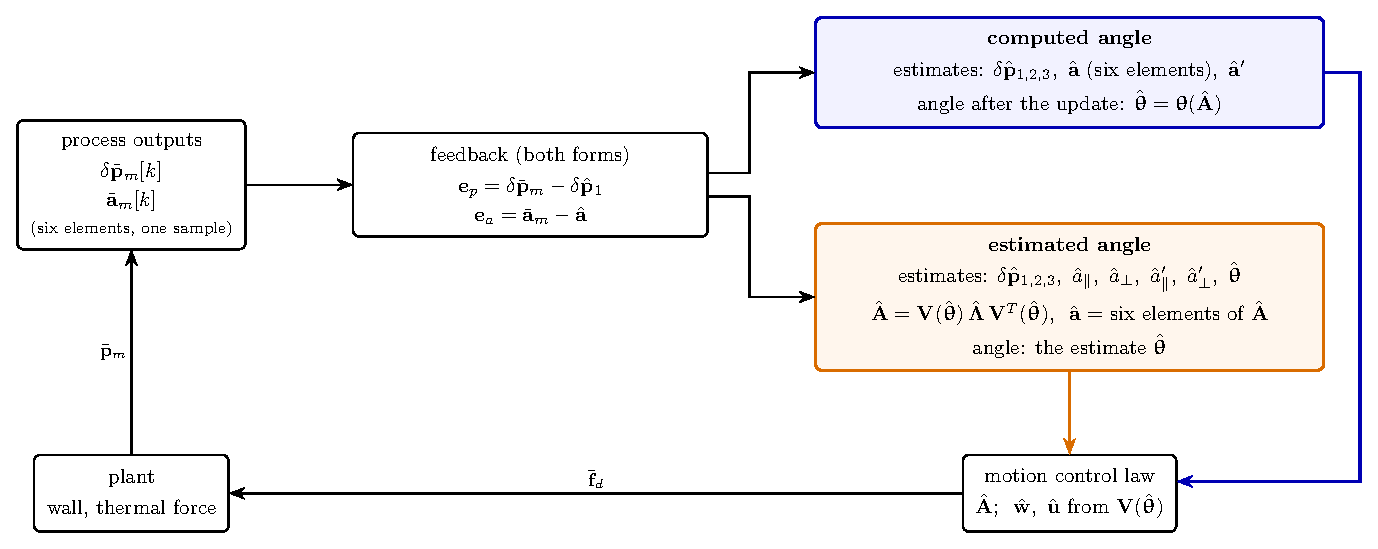
\includegraphics[width=\textwidth]{fig_1025_block.pdf}
\end{center}

%======================================================================
\section{Wall and motion gain matrix}
\setline{bar: normalized (length $/R$, gain $/a_{\mathrm{nom}}$); $\parallel$, $\perp$: parallel, perpendicular to the wall}
\begin{align*}
\V(\bth) &= \begin{bmatrix} \cos\theta_y & \sin\theta_y\sin\theta_x & \sin\theta_y\cos\theta_x \\ 0 & \cos\theta_x & -\sin\theta_x \\ -\sin\theta_y & \cos\theta_y\sin\theta_x & \cos\theta_y\cos\theta_x \end{bmatrix} = [\,\uu\ \ \vv\ \ \ww\,], \qquad \bth = [\,\theta_x\ \ \theta_y\,]^{\T} \\
\ww &= [\,\sin\theta_y\cos\theta_x\ \ \ -\sin\theta_x\ \ \ \cos\theta_y\cos\theta_x\,]^{\T} \\
\Lb &= \mathrm{diag}\big(\apar,\ \apar,\ \aper\big) \\
\Ab &= \V\,\Lb\,\V^{\T} = \apar\,\I + \big(\aper - \apar\big)\,\ww\,\ww^{\T}
\end{align*}
\setline{elements of $\Ab$ and their vector}
\begin{align*}
\Ab &= \begin{bmatrix} \bar a_{xx} & \bar a_{xy} & \bar a_{xz} \\ \bar a_{xy} & \bar a_{yy} & \bar a_{yz} \\ \bar a_{xz} & \bar a_{yz} & \bar a_{zz} \end{bmatrix} \\
\av &= [\,\bar a_{xx}\ \ \bar a_{yy}\ \ \bar a_{zz}\ \ \bar a_{xy}\ \ \bar a_{xz}\ \ \bar a_{yz}\,]^{\T}
\end{align*}
\setline{change along the surface normal, $h$ = distance to the wall}
\begin{align*}
\Ab' &= \frac{\mathrm d\Ab}{\mathrm dh}, \qquad \av' = \frac{\mathrm d\av}{\mathrm dh}
\end{align*}

%======================================================================
\clearpage
\section{Process}
\setline{hat: estimate, normalized as the bar quantity}
\begin{align*}
\bar{\mathbf p}[k+1] &= \bar{\mathbf p}[k] + \Ab\,\big(\bar{\mathbf f}_d[k] + \bar{\mathbf f}_T[k]\big) \\
\dpb[k] &= \bar{\mathbf p}_d[k] - \bar{\mathbf p}[k] \\
\bar{\mathbf p}_m[k] &= \bar{\mathbf p}[k-d] + \bar{\mathbf n}_p[k] \\
\dpb_m[k] &= \bar{\mathbf p}_d[k-d] - \bar{\mathbf p}_m[k] \\
\hat{\mathbf p}[k] &= \bar{\mathbf p}_m[k] + \sum_{i=1}^{d} \Ah[k-i]\,\bar{\mathbf f}_d[k-i] \\
\bar{\mathbf f}_d[k] &= \Ah^{-1}[k]\,\Big\{\bar{\mathbf p}_d[k+1] - \hat{\mathbf p}[k] - \lc\,\big(\bar{\mathbf p}_d[k] - \hat{\mathbf p}[k]\big)\Big\}
\end{align*}
\setline{dynamics of tracking error}
\begin{align*}
\dpb[k+1] &= \lc\,\dpb[k] - \big(\Ab - \Ah[k]\big)\,\Fd[k] - \bep[k] \\
\Fd[k] &= \bar{\mathbf f}_d[k] + (1-\lc)\sum_{i=1}^{d} \bar{\mathbf f}_d[k-i] \\
\bep[k] &= \Ab\,\bar{\mathbf f}_T[k] + (1-\lc)\sum_{i=1}^{d} \Ab\,\bar{\mathbf f}_T[k-i] - (1-\lc)\,\bar{\mathbf n}_p[k]
\end{align*}
\setline{$F_x, F_y, F_z$: elements of $\Fd[k]$}
\begin{align*}
\big(\Ab - \Ah\big)\,\Fd &=
\begin{bmatrix}
(\bar a_{xx} - \hat a_{xx})\,F_x + (\bar a_{xy} - \hat a_{xy})\,F_y + (\bar a_{xz} - \hat a_{xz})\,F_z \\
(\bar a_{xy} - \hat a_{xy})\,F_x + (\bar a_{yy} - \hat a_{yy})\,F_y + (\bar a_{yz} - \hat a_{yz})\,F_z \\
(\bar a_{xz} - \hat a_{xz})\,F_x + (\bar a_{yz} - \hat a_{yz})\,F_y + (\bar a_{zz} - \hat a_{zz})\,F_z
\end{bmatrix}
= \mathbf G_a[k]\,\big(\av - \ah\big) \\
\mathbf G_a[k] &= \GA
\end{align*}
\setline{change of the motion gain matrix with the motion along the surface normal}
\begin{align*}
\Mb[k] &= \Delta\bar{\mathbf p}_d[k] + (1-\lc)\,\dpb_3[k] \\
\Ab[k+1] &= \Ab[k] + \ww^{\T}\Big(\Mb[k] + \big(\Ab - \Ah[k]\big)\,\Fd[k] + \bep[k]\Big)\,\Ab'[k]
\end{align*}

%======================================================================
\clearpage
\section{Process outputs}
\setline{subscript $m$: measured; one sample per step}
\begin{align*}
\dpb_{md}[k+1] &= a_{\mathrm{pd}}\,\dpb_m[k] + (1-a_{\mathrm{pd}})\,\dpb_{md}[k] \\
\dpb_{mr}[k] &= \dpb_m[k] - \dpb_{md}[k] \\
\E\big[\dpb_{mr}\,\dpb_{mr}^{\T}\big] &= \CK\,\Ab + C_n\,\Sn \\
\Am[k] &= \frac{\dpb_{mr}[k]\,\dpb_{mr}^{\T}[k] - C_n\,\Sn}{\CK} \\
\E\big[\Am\big] &= \Ab \\
\am[k] &= [\,\bar a_{m,xx}\ \ \bar a_{m,yy}\ \ \bar a_{m,zz}\ \ \bar a_{m,xy}\ \ \bar a_{m,xz}\ \ \bar a_{m,yz}\,]^{\T}
\end{align*}

%======================================================================
\section{Angle of a gain matrix}
\setline{$\theta_x = 0$}
\begin{align*}
\bar a_{xx} &= \apar\cos^2\theta_y + \aper\sin^2\theta_y \\
\bar a_{zz} &= \apar\sin^2\theta_y + \aper\cos^2\theta_y \\
\bar a_{xz} &= -\big(\apar - \aper\big)\,\sin\theta_y\cos\theta_y \\
\bar a_{xx} - \bar a_{zz} &= \big(\apar - \aper\big)\cos 2\theta_y \\
-2\,\bar a_{xz} &= \big(\apar - \aper\big)\sin 2\theta_y \\
\tan 2\theta_y &= \frac{-2\,\bar a_{xz}}{\bar a_{xx} - \bar a_{zz}}
\end{align*}
\setline{three axes: $\varphi_{yz}$ = angle of $\ww$ in the $y$--$z$ plane}
\begin{align*}
\tan 2\theta_y &= \frac{-2\,\bar a_{xz}}{\bar a_{xx} - \bar a_{zz}} \\
\tan 2\varphi_{yz} &= \frac{-2\,\bar a_{yz}}{\bar a_{yy} - \bar a_{zz}} \\
\theta_x &= -\arctan\big(\tan\varphi_{yz}\,\cos\theta_y\big) \\
\bth(\Ab) &= [\,\theta_x\ \ \theta_y\,]^{\T}
\end{align*}

%======================================================================
\clearpage
\section{Computed angle}
\setline{true state}
\begin{align*}
\dpb_1[k+1] &= \dpb_2[k] \\
\dpb_2[k+1] &= \dpb_3[k] \\
\dpb_3[k+1] &= \lc\,\dpb_3[k] - \mathbf G_a[k]\,\big(\av[k] - \ah[k]\big) - \bep[k] \\
\av[k+1] &= \av[k] + \av'[k]\,\ww^{\T}\Big(\Mb[k] + \mathbf G_a[k]\,\big(\av[k] - \ah[k]\big) + \bep[k]\Big) \\
\av'[k+1] &= \av'[k]
\end{align*}
\begin{align*}
&\big[\,\dpb_1^{\T}\ \ \dpb_2^{\T}\ \ \dpb_3^{\T}\ \ \av^{\T}\ \ \av'^{\T}\,\big]^{\T} \qquad (21 \times 1,\ d = 2)
\end{align*}
\setline{process outputs, their estimates and the output matrix}
\begin{align*}
\mathbf y_m[k] &= \begin{bmatrix} \dpb_m[k] \\ \am[k] \end{bmatrix}, \qquad
\hat{\mathbf y}[k] = \begin{bmatrix} \dph_1[k] \\ \ah[k] \end{bmatrix}, \qquad
\mathbf H = \begin{bmatrix} \I_3 & \mathbf 0 & \mathbf 0 & \mathbf 0 & \mathbf 0 \\ \mathbf 0 & \mathbf 0 & \mathbf 0 & \I_6 & \mathbf 0 \end{bmatrix}
\end{align*}
\setline{feedback: measured $-$ estimate}
\begin{align*}
\mathbf e_p[k] &= \dpb_m[k] - \dph_1[k] \\
\mathbf e_a[k] &= \am[k] - \ah[k]
\end{align*}
\setline{estimator; $\wh[k]$ from $\hat\bth[k] = \bth(\Ah[k])$}
\begin{align*}
\Mh[k] &= \Delta\bar{\mathbf p}_d[k] + (1-\lc)\,\dph_3[k] \\
\dph_1[k+1] &= \dph_2[k] + \mathbf L_1[k] \eyl{} \\
\dph_2[k+1] &= \dph_3[k] + \mathbf L_2[k] \eyl{} \\
\dph_3[k+1] &= \lc\,\dph_3[k] + \mathbf L_3[k] \eyl{} \\
\ah[k+1] &= \ah[k] + \hat{\mathbf a}'[k]\,\wh^{\T}[k]\,\Mh[k] + \mathbf L_4[k] \eyl{} \\
\hat{\mathbf a}'[k+1] &= \hat{\mathbf a}'[k] + \mathbf L_5[k] \eyl{}
\end{align*}
\setline{estimator feedback matrix and error covariance}
\begin{align*}
\mathbf L[k] &= \mathbf P^f[k]\,\mathbf H^{\T}\big(\mathbf H\,\mathbf P^f[k]\,\mathbf H^{\T} + \mathbf R[k]\big)^{-1} \\
\mathbf P[k] &= \big(\I - \mathbf L[k]\,\mathbf H\big)\,\mathbf P^f[k]
\end{align*}
\setline{estimation error: true $-$ estimate}
\begin{align*}
\mathbf e[k] &= \big[\,\big(\dpb_1 - \dph_1\big)^{\T}\ \ \big(\dpb_2 - \dph_2\big)^{\T}\ \ \big(\dpb_3 - \dph_3\big)^{\T}\ \ \big(\av - \ah\big)^{\T}\ \ \big(\av' - \hat{\mathbf a}'\big)^{\T}\,\big]^{\T}
\end{align*}
\setline{dynamics of estimation errors, first order, without the feedback terms}
\begin{align*}
\dpb_1[k+1] - \dph_1[k+1] &= \dpb_2[k] - \dph_2[k] \\
\dpb_2[k+1] - \dph_2[k+1] &= \dpb_3[k] - \dph_3[k] \\
\dpb_3[k+1] - \dph_3[k+1] &= \lc\,\big(\dpb_3[k] - \dph_3[k]\big) - \mathbf G_a[k]\,\big(\av[k] - \ah[k]\big) - \bep[k] \\
\av[k+1] - \ah[k+1] &= \big(\av[k] - \ah[k]\big) + \big(\av'[k] - \hat{\mathbf a}'[k]\big)\,\wh^{\T}[k]\,\Mh[k] \\
&\quad + \hat{\mathbf a}'[k]\,\wh^{\T}[k]\Big((1-\lc)\big(\dpb_3[k] - \dph_3[k]\big) + \mathbf G_a[k]\,\big(\av[k] - \ah[k]\big) + \bep[k]\Big) \\
\av'[k+1] - \hat{\mathbf a}'[k+1] &= \av'[k] - \hat{\mathbf a}'[k]
\end{align*}
\begin{align*}
\mathbf e[k+1] &= \mathbf F_e[k]\,\mathbf e[k] + \big[\,\mathbf 0\ \ \mathbf 0\ \ -\bep^{\T}[k]\ \ \big(\hat{\mathbf a}'[k]\,\wh^{\T}[k]\,\bep[k]\big)^{\T}\ \ \mathbf 0\,\big]^{\T} \\
\mathbf F_e[k] &=
\begin{bmatrix}
\mathbf 0 & \I_3 & \mathbf 0 & \mathbf 0 & \mathbf 0 \\
\mathbf 0 & \mathbf 0 & \I_3 & \mathbf 0 & \mathbf 0 \\
\mathbf 0 & \mathbf 0 & \lc\,\I_3 & -\mathbf G_a[k] & \mathbf 0 \\
\mathbf 0 & \mathbf 0 & (1-\lc)\,\hat{\mathbf a}'[k]\,\wh^{\T}[k] & \I_6 + \hat{\mathbf a}'[k]\,\wh^{\T}[k]\,\mathbf G_a[k] & \big(\wh^{\T}[k]\,\Mh[k]\big)\,\I_6 \\
\mathbf 0 & \mathbf 0 & \mathbf 0 & \mathbf 0 & \I_6
\end{bmatrix}
\end{align*}
\setline{process noise and error covariance}
\begin{align*}
\mathbf Q[k] &= \E\Big[\big[\,\mathbf 0\ \ \mathbf 0\ \ -\bep^{\T}\ \ \big(\hat{\mathbf a}'\,\wh^{\T}\bep\big)^{\T}\ \ \mathbf 0\,\big]^{\T}
\big[\,\mathbf 0\ \ \mathbf 0\ \ -\bep^{\T}\ \ \big(\hat{\mathbf a}'\,\wh^{\T}\bep\big)^{\T}\ \ \mathbf 0\,\big]\Big]
+ \mathrm{diag}\big(\mathbf 0,\ \mathbf 0,\ \mathbf 0,\ \mathbf 0,\ \mathbf Q_{a'}[k]\big) \\
\mathbf P^f[k+1] &= \mathbf F_e[k]\,\mathbf P[k]\,\mathbf F_e^{\T}[k] + \mathbf Q[k]
\end{align*}
\setline{angle: computed from the estimate}
\begin{align*}
\hat\bth[k] &= \bth\big(\Ah[k]\big), \qquad \Vh[k] = \V\big(\hat\bth[k]\big) = [\,\hat\uu\ \ \hat\vv\ \ \wh\,]
\end{align*}

%======================================================================
\clearpage
\section{Estimated angle}
\setline{gain matrix from two gains and the angle; plane wall: constant angle}
\begin{align*}
\Ab &= \V(\bth)\,\Lb\,\V^{\T}(\bth) = \apar\,\I + \big(\aper - \apar\big)\,\ww\,\ww^{\T} \\
\Ab' &= \apar'\,\big(\I - \ww\,\ww^{\T}\big) + \aper'\,\ww\,\ww^{\T} \\
\Ah[k] &= \V\big(\hat\bth[k]\big)\,\hat{\bm\Lambda}[k]\,\V^{\T}\big(\hat\bth[k]\big), \qquad \hat{\bm\Lambda}[k] = \mathrm{diag}\big(\hat a_\parallel[k],\ \hat a_\parallel[k],\ \hat a_\perp[k]\big)
\end{align*}
\setline{first-order change of $\Ab$; $\partial\av/\partial(\cdot)$: the six elements of $\partial\Ab/\partial(\cdot)$}
\begin{align*}
\frac{\partial\Ab}{\partial\apar} &= \I - \ww\,\ww^{\T} \\
\frac{\partial\Ab}{\partial\aper} &= \ww\,\ww^{\T} \\
\frac{\partial\Ab}{\partial\theta_x} &= \big(\aper - \apar\big)\Big(\frac{\partial\ww}{\partial\theta_x}\,\ww^{\T} + \ww\,\frac{\partial\ww^{\T}}{\partial\theta_x}\Big), \qquad
\frac{\partial\Ab}{\partial\theta_y} = \big(\aper - \apar\big)\Big(\frac{\partial\ww}{\partial\theta_y}\,\ww^{\T} + \ww\,\frac{\partial\ww^{\T}}{\partial\theta_y}\Big) \\
\frac{\partial\ww}{\partial\bth} &= \Big[\,\frac{\partial\ww}{\partial\theta_x}\ \ \frac{\partial\ww}{\partial\theta_y}\,\Big] =
\begin{bmatrix}
-\sin\theta_y\sin\theta_x & \cos\theta_y\cos\theta_x \\
-\cos\theta_x & 0 \\
-\cos\theta_y\sin\theta_x & -\sin\theta_y\cos\theta_x
\end{bmatrix} \\
\av - \ah &= \frac{\partial\av}{\partial\apar}\,\big(\apar - \hat a_\parallel\big) + \frac{\partial\av}{\partial\aper}\,\big(\aper - \hat a_\perp\big) + \frac{\partial\av}{\partial\bth}\,\big(\bth - \hat\bth\big)
\end{align*}
\setline{true state}
\begin{align*}
\dpb_1[k+1] &= \dpb_2[k] \\
\dpb_2[k+1] &= \dpb_3[k] \\
\dpb_3[k+1] &= \lc\,\dpb_3[k] - \mathbf G_a[k]\,\big(\av[k] - \ah[k]\big) - \bep[k] \\
\apar[k+1] &= \apar[k] + \apar'[k]\,\ww^{\T}\Big(\Mb[k] + \mathbf G_a[k]\,\big(\av[k] - \ah[k]\big) + \bep[k]\Big) \\
\aper[k+1] &= \aper[k] + \aper'[k]\,\ww^{\T}\Big(\Mb[k] + \mathbf G_a[k]\,\big(\av[k] - \ah[k]\big) + \bep[k]\Big) \\
\apar'[k+1] &= \apar'[k] \\
\aper'[k+1] &= \aper'[k] \\
\bth[k+1] &= \bth[k]
\end{align*}
\begin{align*}
&\big[\,\dpb_1^{\T}\ \ \dpb_2^{\T}\ \ \dpb_3^{\T}\ \ \apar\ \ \aper\ \ \apar'\ \ \aper'\ \ \bth^{\T}\,\big]^{\T} \qquad (15 \times 1,\ d = 2)
\end{align*}
\setline{process outputs, their estimates and the output matrix (derivatives at the estimate)}
\begin{align*}
\mathbf y_m[k] &= \begin{bmatrix} \dpb_m[k] \\ \am[k] \end{bmatrix}, \qquad
\hat{\mathbf y}[k] = \begin{bmatrix} \dph_1[k] \\ \ah[k] \end{bmatrix} \\
\mathbf H[k] &= \begin{bmatrix} \I_3 & \mathbf 0 & \mathbf 0 & \mathbf 0 & \mathbf 0 & \mathbf 0 & \mathbf 0 & \mathbf 0 \\
\mathbf 0 & \mathbf 0 & \mathbf 0 & \dfrac{\partial\av}{\partial\apar} & \dfrac{\partial\av}{\partial\aper} & \mathbf 0 & \mathbf 0 & \dfrac{\partial\av}{\partial\bth} \end{bmatrix}
\end{align*}
\setline{feedback: measured $-$ estimate}
\begin{align*}
\mathbf e_p[k] &= \dpb_m[k] - \dph_1[k] \\
\mathbf e_a[k] &= \am[k] - \ah[k]
\end{align*}
\setline{estimator; $\wh[k]$ from the estimate $\hat\bth[k]$; $\mathbf L[k]$, $\mathbf P[k]$ as in Section 5}
\begin{align*}
\Mh[k] &= \Delta\bar{\mathbf p}_d[k] + (1-\lc)\,\dph_3[k] \\
\dph_1[k+1] &= \dph_2[k] + \mathbf L_1[k] \eyl{} \\
\dph_2[k+1] &= \dph_3[k] + \mathbf L_2[k] \eyl{} \\
\dph_3[k+1] &= \lc\,\dph_3[k] + \mathbf L_3[k] \eyl{} \\
\hat a_\parallel[k+1] &= \hat a_\parallel[k] + \hat a'_\parallel[k]\,\wh^{\T}[k]\,\Mh[k] + \mathbf L_4[k] \eyl{} \\
\hat a_\perp[k+1] &= \hat a_\perp[k] + \hat a'_\perp[k]\,\wh^{\T}[k]\,\Mh[k] + \mathbf L_5[k] \eyl{} \\
\hat a'_\parallel[k+1] &= \hat a'_\parallel[k] + \mathbf L_6[k] \eyl{} \\
\hat a'_\perp[k+1] &= \hat a'_\perp[k] + \mathbf L_7[k] \eyl{} \\
\hat\bth[k+1] &= \hat\bth[k] + \mathbf L_8[k] \eyl{}
\end{align*}
\setline{estimation error: true $-$ estimate}
\begin{align*}
\mathbf e[k] &= \big[\,\big(\dpb_1 - \dph_1\big)^{\T}\ \ \big(\dpb_2 - \dph_2\big)^{\T}\ \ \big(\dpb_3 - \dph_3\big)^{\T}\ \ \apar - \hat a_\parallel\ \ \aper - \hat a_\perp\ \ \apar' - \hat a'_\parallel\ \ \aper' - \hat a'_\perp\ \ \big(\bth - \hat\bth\big)^{\T}\,\big]^{\T}
\end{align*}
\setline{dynamics of estimation errors, first order, without the feedback terms}
\begin{align*}
\dpb_1[k+1] - \dph_1[k+1] &= \dpb_2[k] - \dph_2[k] \\
\dpb_2[k+1] - \dph_2[k+1] &= \dpb_3[k] - \dph_3[k] \\
\dpb_3[k+1] - \dph_3[k+1] &= \lc\,\big(\dpb_3[k] - \dph_3[k]\big) - \mathbf G_a[k]\,\big(\av[k] - \ah[k]\big) - \bep[k] \\
\apar[k+1] - \hat a_\parallel[k+1] &= \big(\apar[k] - \hat a_\parallel[k]\big) + \big(\apar'[k] - \hat a'_\parallel[k]\big)\,\wh^{\T}[k]\,\Mh[k] + \hat a'_\parallel[k]\,\Mh^{\T}[k]\,\frac{\partial\ww}{\partial\bth}\,\big(\bth[k] - \hat\bth[k]\big) \\
&\quad + \hat a'_\parallel[k]\,\wh^{\T}[k]\Big((1-\lc)\big(\dpb_3[k] - \dph_3[k]\big) + \mathbf G_a[k]\,\big(\av[k] - \ah[k]\big) + \bep[k]\Big) \\
\aper[k+1] - \hat a_\perp[k+1] &= \big(\aper[k] - \hat a_\perp[k]\big) + \big(\aper'[k] - \hat a'_\perp[k]\big)\,\wh^{\T}[k]\,\Mh[k] + \hat a'_\perp[k]\,\Mh^{\T}[k]\,\frac{\partial\ww}{\partial\bth}\,\big(\bth[k] - \hat\bth[k]\big) \\
&\quad + \hat a'_\perp[k]\,\wh^{\T}[k]\Big((1-\lc)\big(\dpb_3[k] - \dph_3[k]\big) + \mathbf G_a[k]\,\big(\av[k] - \ah[k]\big) + \bep[k]\Big) \\
\apar'[k+1] - \hat a'_\parallel[k+1] &= \apar'[k] - \hat a'_\parallel[k] \\
\aper'[k+1] - \hat a'_\perp[k+1] &= \aper'[k] - \hat a'_\perp[k] \\
\bth[k+1] - \hat\bth[k+1] &= \bth[k] - \hat\bth[k]
\end{align*}
\begin{align*}
\mathbf e[k+1] &= \mathbf F_e[k]\,\mathbf e[k] + \big[\,\mathbf 0\ \ \mathbf 0\ \ -\bep^{\T}[k]\ \ \hat a'_\parallel[k]\,\wh^{\T}[k]\,\bep[k]\ \ \hat a'_\perp[k]\,\wh^{\T}[k]\,\bep[k]\ \ 0\ \ 0\ \ \mathbf 0\,\big]^{\T}
\end{align*}
{\small
\begin{align*}
\mathbf F_e[k] &=
\begin{bmatrix}
\mathbf 0 & \I_3 & \mathbf 0 & \mathbf 0 & \mathbf 0 & \mathbf 0 & \mathbf 0 & \mathbf 0 \\
\mathbf 0 & \mathbf 0 & \I_3 & \mathbf 0 & \mathbf 0 & \mathbf 0 & \mathbf 0 & \mathbf 0 \\
\mathbf 0 & \mathbf 0 & \lc\,\I_3 & -\mathbf G_a\dfrac{\partial\av}{\partial\apar} & -\mathbf G_a\dfrac{\partial\av}{\partial\aper} & \mathbf 0 & \mathbf 0 & -\mathbf G_a\dfrac{\partial\av}{\partial\bth} \\[6pt]
\mathbf 0 & \mathbf 0 & (1-\lc)\,\hat a'_\parallel\,\wh^{\T} & 1 + \hat a'_\parallel\,\wh^{\T}\mathbf G_a\dfrac{\partial\av}{\partial\apar} & \hat a'_\parallel\,\wh^{\T}\mathbf G_a\dfrac{\partial\av}{\partial\aper} & \wh^{\T}\Mh & 0 &
\begin{array}{c} \hat a'_\parallel\,\wh^{\T}\mathbf G_a\dfrac{\partial\av}{\partial\bth} \\[14pt] +\ \hat a'_\parallel\,\Mh^{\T}\dfrac{\partial\ww}{\partial\bth} \end{array} \\[22pt]
\mathbf 0 & \mathbf 0 & (1-\lc)\,\hat a'_\perp\,\wh^{\T} & \hat a'_\perp\,\wh^{\T}\mathbf G_a\dfrac{\partial\av}{\partial\apar} & 1 + \hat a'_\perp\,\wh^{\T}\mathbf G_a\dfrac{\partial\av}{\partial\aper} & 0 & \wh^{\T}\Mh &
\begin{array}{c} \hat a'_\perp\,\wh^{\T}\mathbf G_a\dfrac{\partial\av}{\partial\bth} \\[14pt] +\ \hat a'_\perp\,\Mh^{\T}\dfrac{\partial\ww}{\partial\bth} \end{array} \\[22pt]
\mathbf 0 & \mathbf 0 & \mathbf 0 & 0 & 0 & 1 & 0 & \mathbf 0 \\
\mathbf 0 & \mathbf 0 & \mathbf 0 & 0 & 0 & 0 & 1 & \mathbf 0 \\
\mathbf 0 & \mathbf 0 & \mathbf 0 & \mathbf 0 & \mathbf 0 & \mathbf 0 & \mathbf 0 & \I_2
\end{bmatrix}
\end{align*}}
\setline{process noise and error covariance}
\begin{align*}
\mathbf Q[k] &= \E\Big[\big[\,\mathbf 0\ \ \mathbf 0\ \ -\bep^{\T}\ \ \hat a'_\parallel\,\wh^{\T}\bep\ \ \hat a'_\perp\,\wh^{\T}\bep\ \ 0\ \ 0\ \ \mathbf 0\,\big]^{\T}
\big[\,\mathbf 0\ \ \mathbf 0\ \ -\bep^{\T}\ \ \hat a'_\parallel\,\wh^{\T}\bep\ \ \hat a'_\perp\,\wh^{\T}\bep\ \ 0\ \ 0\ \ \mathbf 0\,\big]\Big] \\
&\quad + \mathrm{diag}\big(\mathbf 0,\ \mathbf 0,\ \mathbf 0,\ 0,\ 0,\ \mathbf Q_{a'}[k],\ \mathbf 0\big) \\
\mathbf P^f[k+1] &= \mathbf F_e[k]\,\mathbf P[k]\,\mathbf F_e^{\T}[k] + \mathbf Q[k]
\end{align*}
\setline{angle: the estimate}
\begin{align*}
\Vh[k] &= \V\big(\hat\bth[k]\big) = [\,\hat\uu\ \ \hat\vv\ \ \wh\,]
\end{align*}

%======================================================================
\clearpage
\section{Fixed-point results}
\setline{wall $\theta_y = 20^\circ$, $\theta_x = 0$; probe held at 15 \textmu m (top) and 5 \textmu m (bottom); left computed angle, right estimated angle with $\hat\bth[0] = \mathbf 0$; seed 1 dark, seeds 2--3 light}
\begin{center}
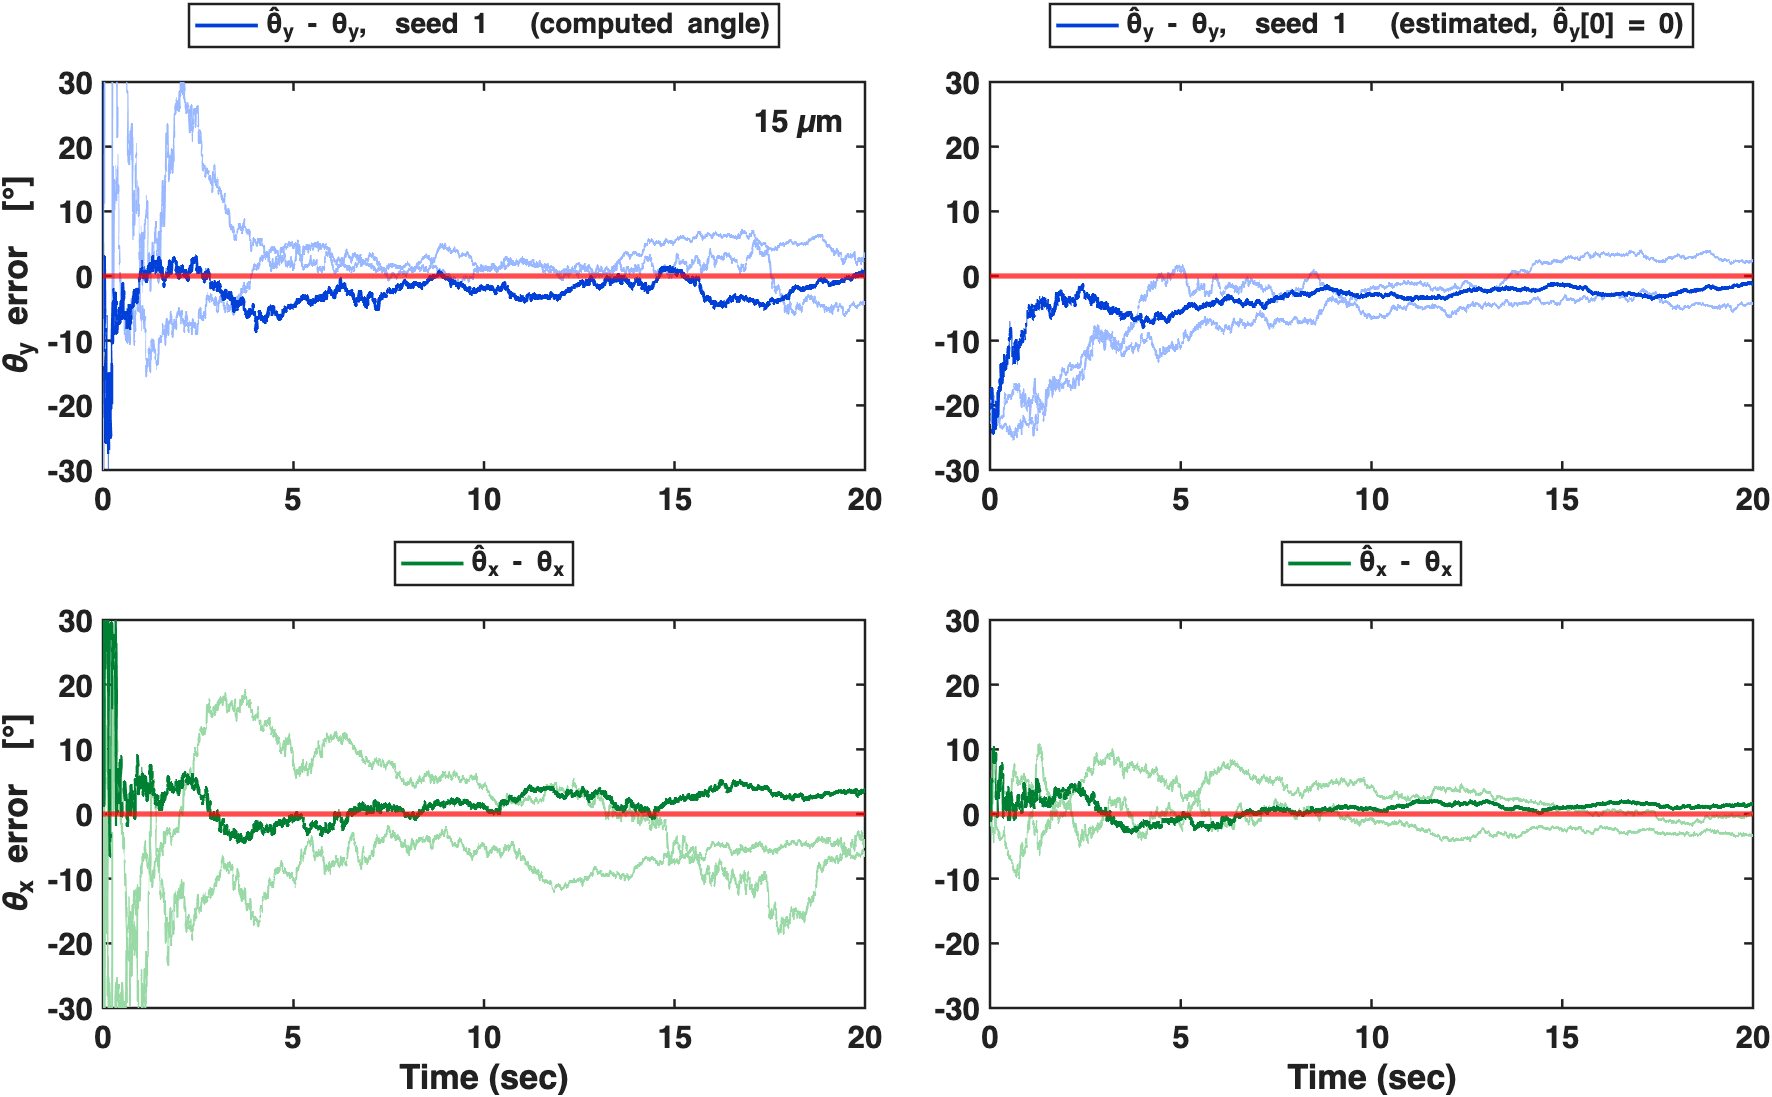
\includegraphics[width=\textwidth]{fig_1025_fixed_15um.png}\\[2pt]
{\small Angle errors at 15 \textmu m over 20 s.}\\[10pt]
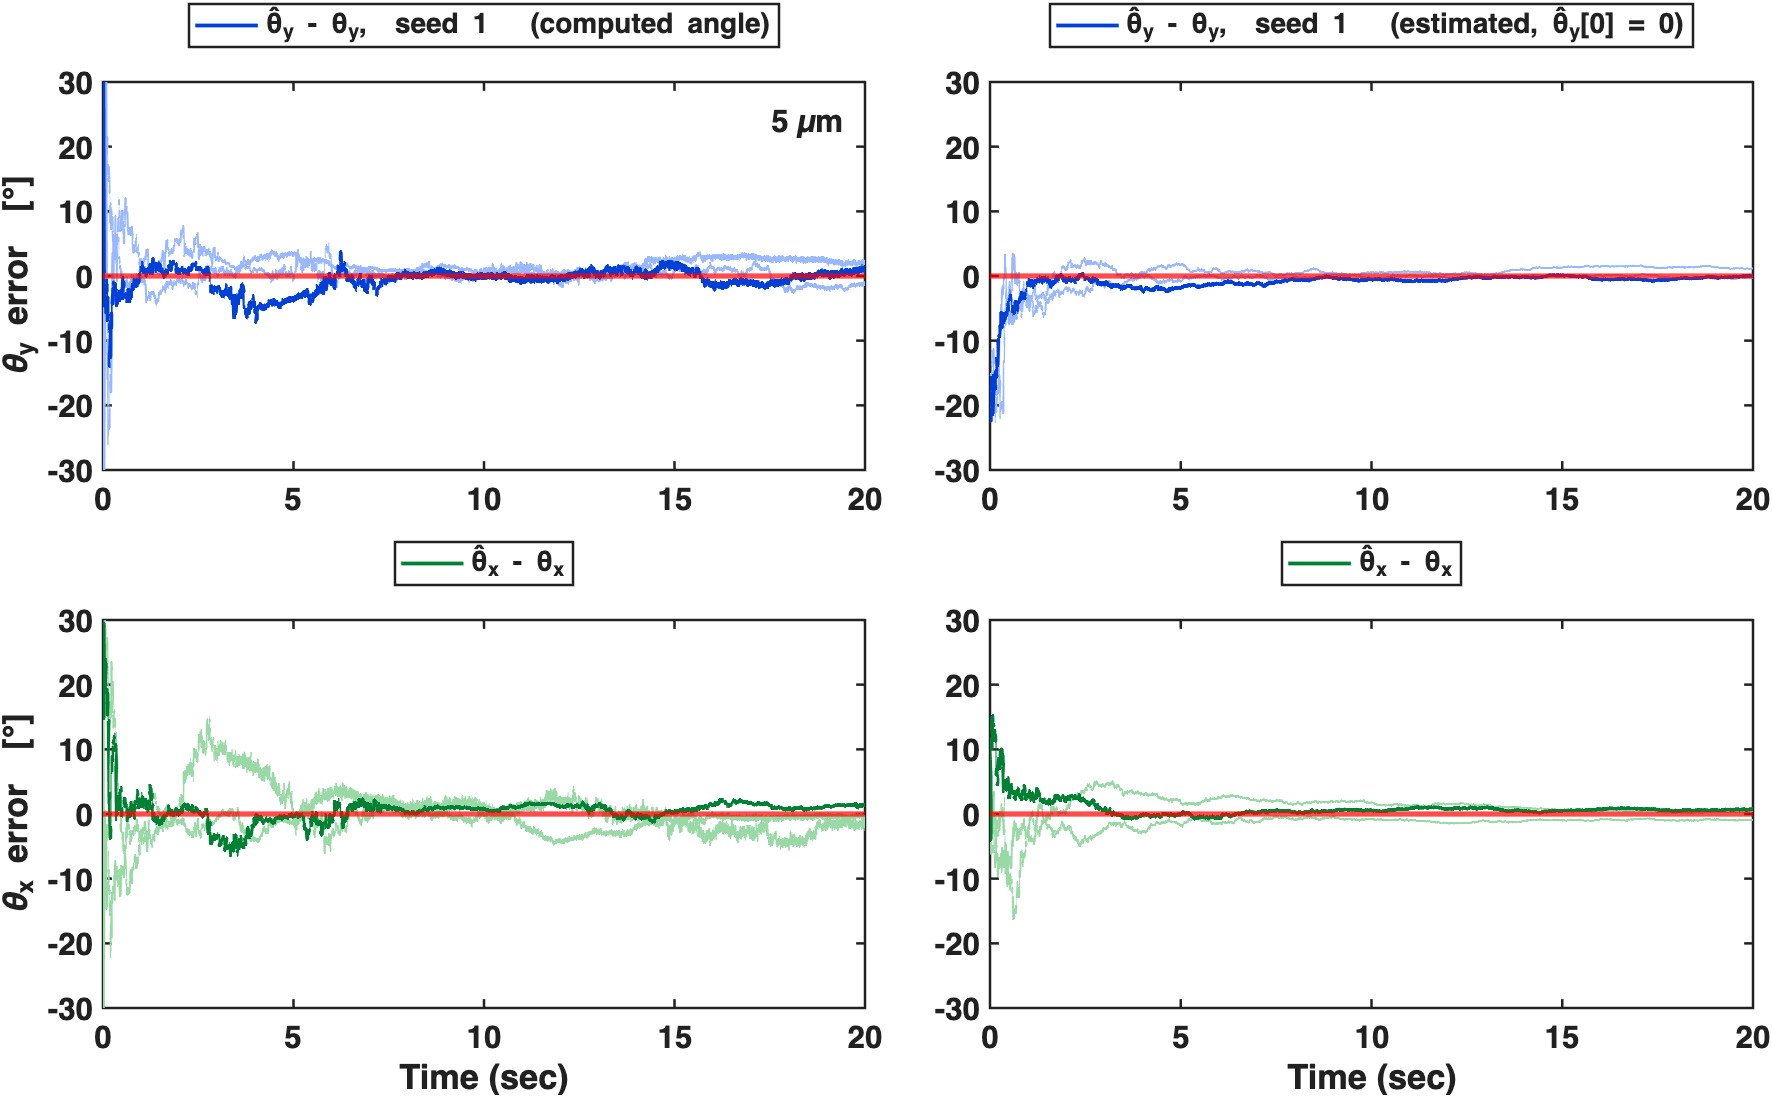
\includegraphics[width=\textwidth]{fig_1025_fixed_5um.png}\\[2pt]
{\small Angle errors at 5 \textmu m over 20 s.}
\end{center}

%======================================================================
\clearpage
\section{Angle error of the computed angle}
\noindent{\small The computed angle is the angle formula evaluated at $\hat{\mathbf A}$, so its error is the error of $\hat{\mathbf A}$ times the sensitivity of the formula.
(1) $\hat{\mathbf A}$: the errors of the three elements in the formula are of the same size at 15 and 5 \textmu m.
(2) Sensitivity: $1/[2(\apar - \aper)]$, larger farther from the wall, so the same error of $\hat{\mathbf A}$ gives a larger angle error and a slower convergence at 15 \textmu m.}
\par\smallskip
\setline{15 \textmu m; lines: 3 seeds with the smallest error; black: $\pm$rms of 10 seeds (solid), $\pm\sqrt{P}$ (dashed)}
\begin{center}
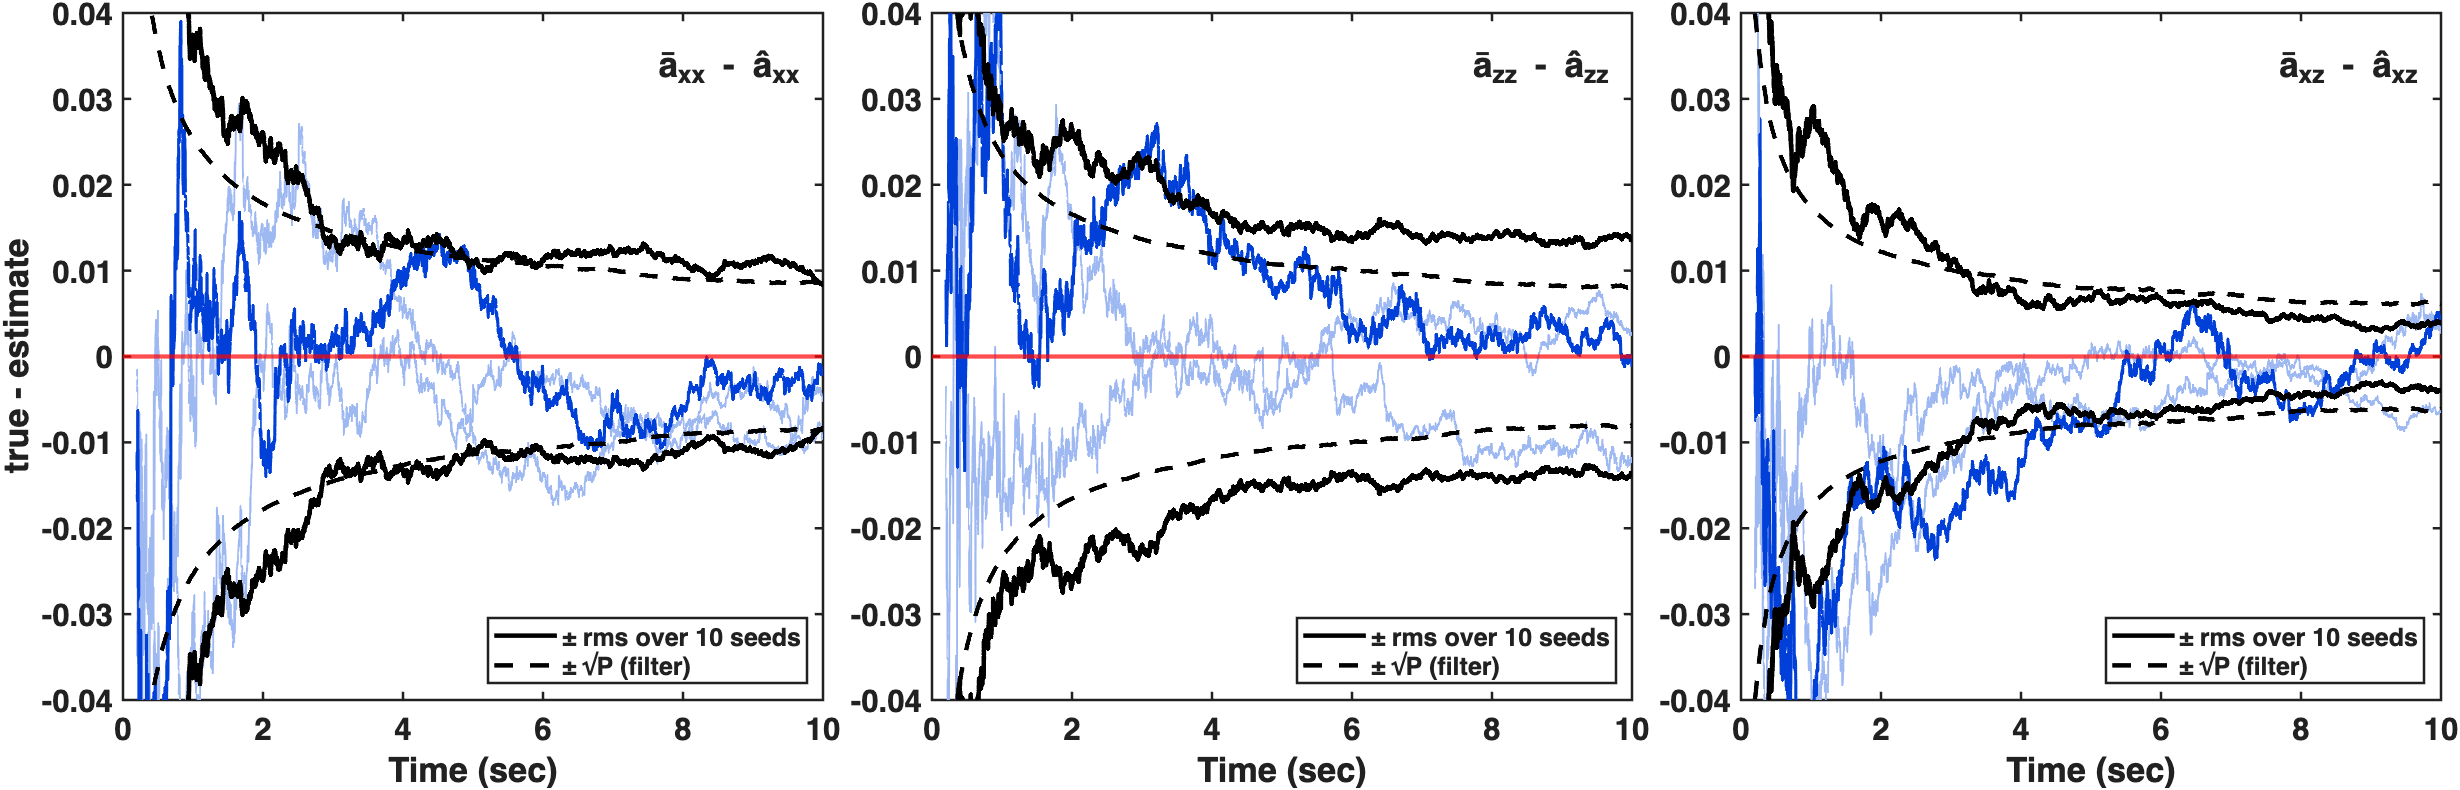
\includegraphics[width=\textwidth]{fig_1025_a_quality.png}
\end{center}
\setline{angle from the gain matrix (Section 4)}
\begin{align*}
\tan 2\theta_y &= \frac{N}{D} \\
N &= -2\,\bar a_{xz} = \big(\apar - \aper\big)\sin 2\theta_y \\
D &= \bar a_{xx} - \bar a_{zz} = \big(\apar - \aper\big)\cos 2\theta_y
\end{align*}
\setline{sensitivity of the angle to $N$ and $D$}
\begin{align*}
\frac{\partial\theta_y}{\partial N} &= \frac{\cos 2\theta_y}{2\big(\apar - \aper\big)}, \qquad
\frac{\partial\theta_y}{\partial D} = \frac{-\sin 2\theta_y}{2\big(\apar - \aper\big)}
\end{align*}
\setline{$e_N = N - \hat N$, $e_D = D - \hat D$; $e(t)$: rms of $e_N$, $e_D$}
\begin{align*}
\theta_y - \hat\theta_y &\approx \frac{\cos 2\theta_y\,e_N - \sin 2\theta_y\,e_D}{2\big(\apar - \aper\big)} \\
\mathrm{rms}\big(\theta_y - \hat\theta_y\big) &\approx \frac{e(t)}{2\big(\apar - \aper\big)}
\end{align*}
\clearpage
\setline{$\apar - \aper$ = 0.083 (15 \textmu m), 0.230 (5 \textmu m); left: $e(t)$, dashed $2(\apar - \aper)\tan 5^\circ$; right: simulation, dashed $e(t)/[2(\apar - \aper)]$}
\begin{center}
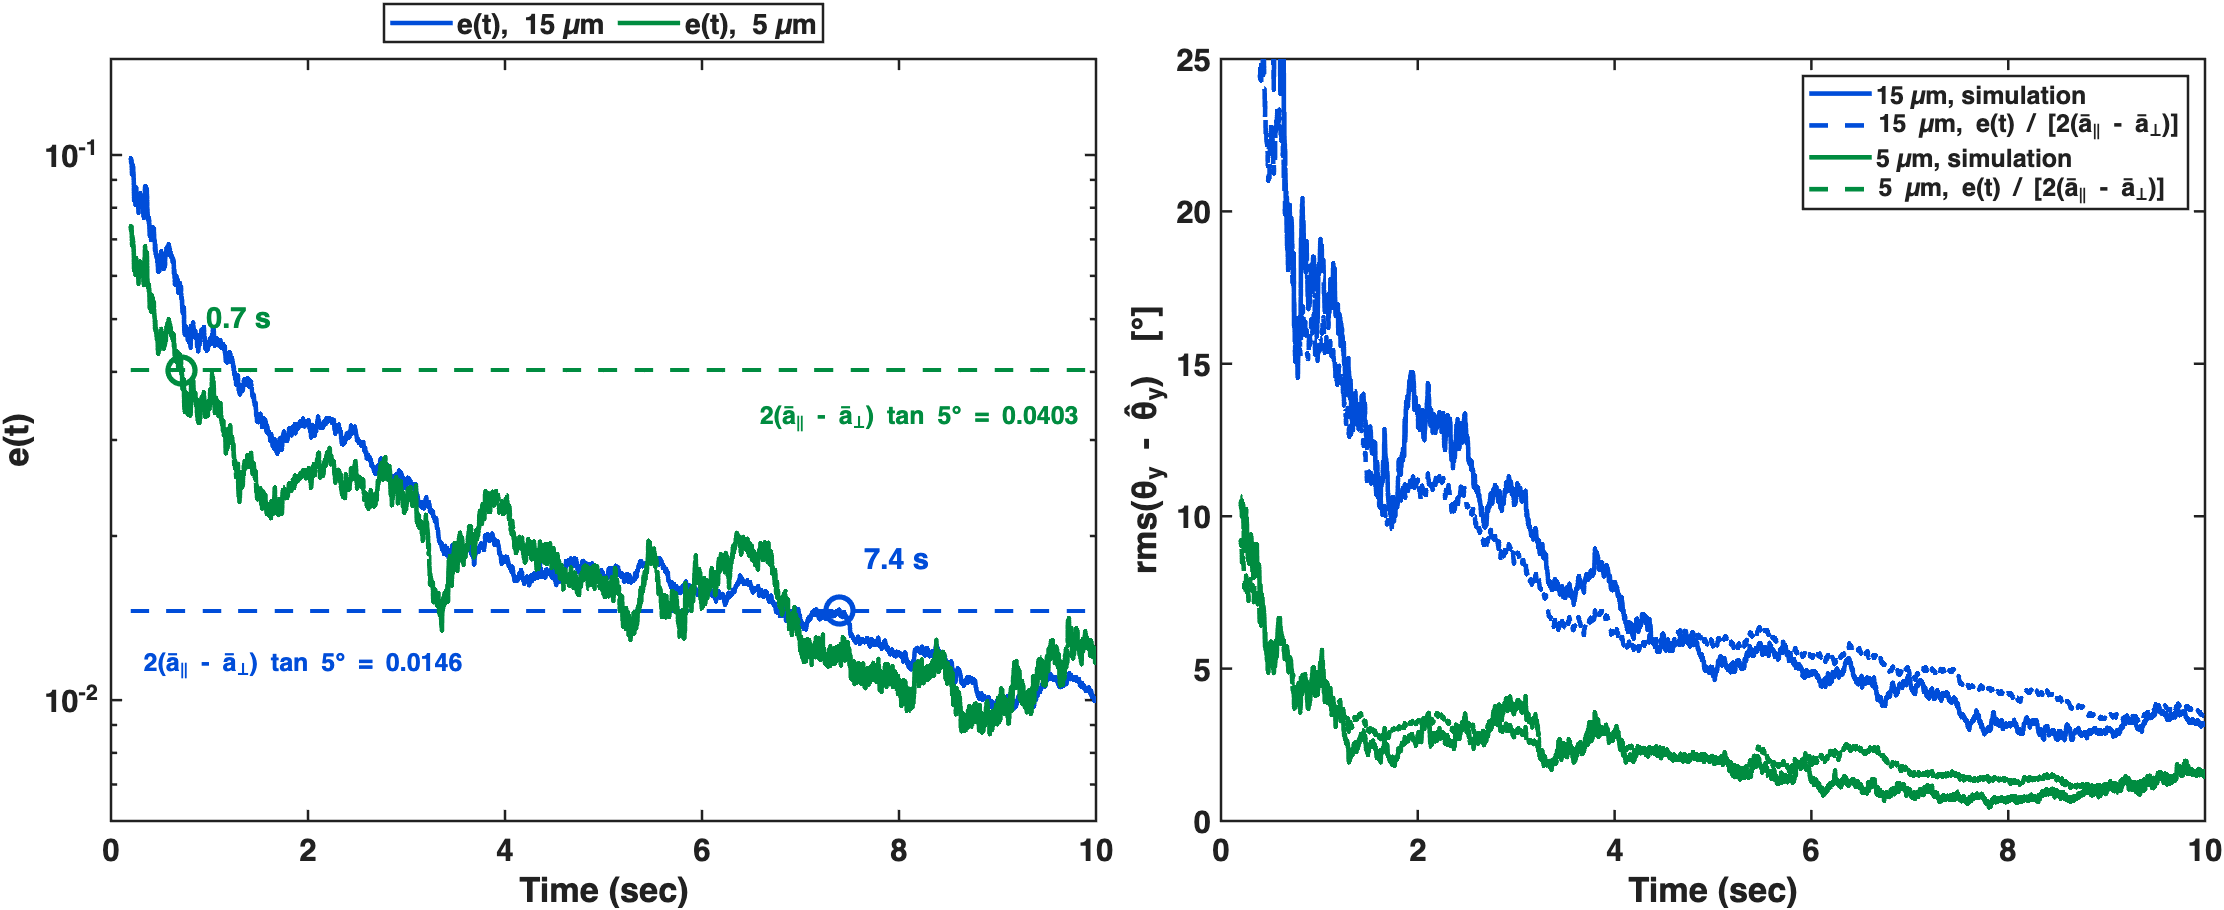
\includegraphics[width=\textwidth]{fig_1025_angle_err.png}\\[2pt]
{\small Same error size $e(t)$ at both heights; the angle error is $e(t)/[2(\apar - \aper)]$.}
\end{center}

%======================================================================
\clearpage
\section{Angle error of the estimated angle}
\noindent{\small The estimated angle reads the angle from the same elements through the angle columns of $\mathbf H$, whose size is $2(\apar - \aper)$.
(1) The angle information per step is proportional to $(\apar - \aper)^2$, so $\sqrt{P_{\theta_y}}$ follows the same $e(t)/[2(\apar - \aper)]$ as the computed angle.
(2) In addition, the initial value is kept with the weight $P_{\theta_y}(t)/P_{\theta_y}(0)$: with little information the estimate stays near the initial value instead of jumping.}
\par\smallskip
\setline{angle columns of $\mathbf H$ for $N$ and $D$ (Section 6)}
\begin{align*}
\frac{\partial N}{\partial\theta_y} &= 2\big(\apar - \aper\big)\cos 2\theta_y, \qquad
\frac{\partial D}{\partial\theta_y} = -2\big(\apar - \aper\big)\sin 2\theta_y
\end{align*}
\setline{uncertainty of the estimated angle}
\begin{align*}
\sqrt{P_{\theta_y}(t)} &\approx \frac{e(t)}{2\big(\apar - \aper\big)}
\end{align*}
\setline{error: initial residual and noise}
\begin{align*}
\theta_y - \hat\theta_y &\approx \frac{P_{\theta_y}(t)}{P_{\theta_y}(0)}\,\big(\theta_y - \hat\theta_y(0)\big) + \text{noise of size } \sqrt{P_{\theta_y}(t)}
\end{align*}
\setline{$\hat\theta_y(0) = 0$, $\sqrt{P_{\theta_y}(0)} = 10^\circ$, wall $20^\circ$; 15 and 5 \textmu m, seeds 1--10; left: $\sqrt{P_{\theta_y}}$ (solid), $e(t)/[2(\apar - \aper)]$ of the computed angle (dashed); right: simulation (solid), initial residual and $\sqrt{P_{\theta_y}}$ (dashed)}
\begin{center}
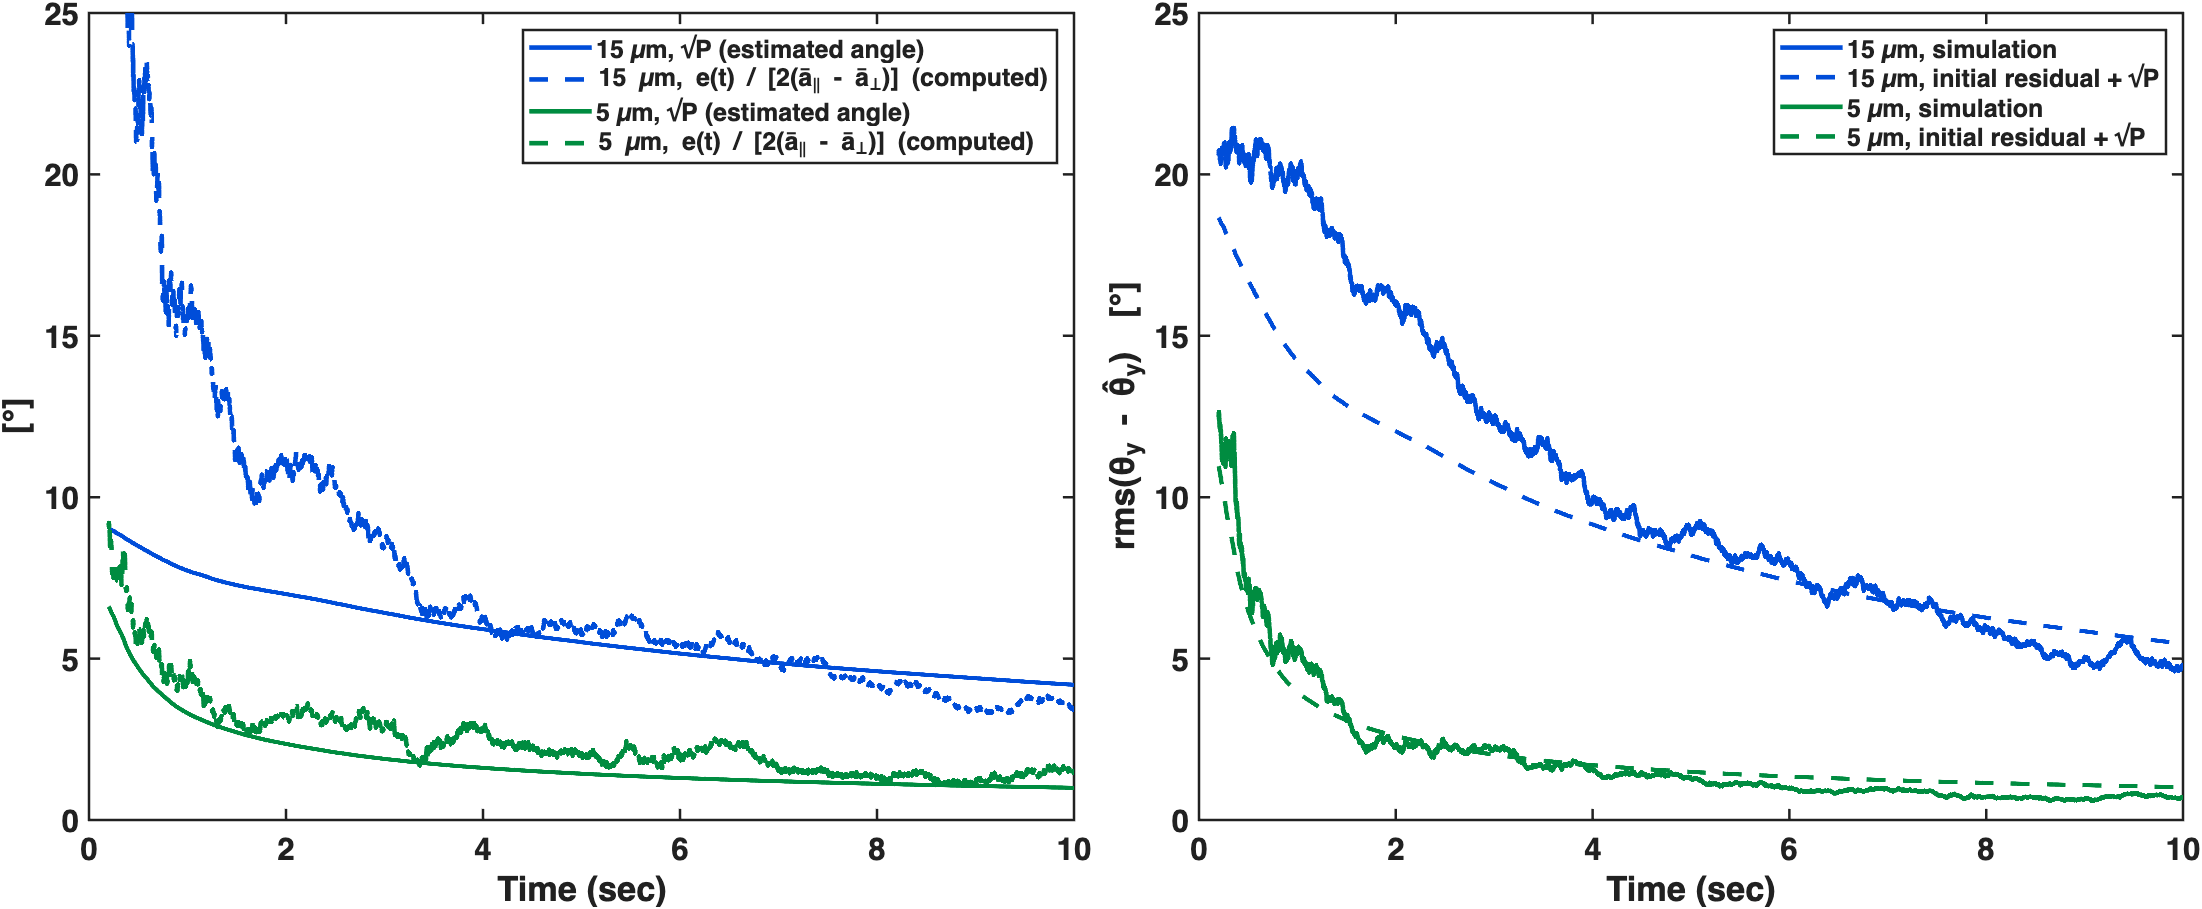
\includegraphics[width=\textwidth]{fig_1025_est_slow.png}\\[2pt]
{\small Same information limit as the computed angle; the remaining error is the initial value.}
\end{center}

\end{document}
